% Options for packages loaded elsewhere
\PassOptionsToPackage{unicode}{hyperref}
\PassOptionsToPackage{hyphens}{url}
\documentclass[
]{article}
\usepackage{xcolor}
\usepackage[margin=1in]{geometry}
\usepackage{amsmath,amssymb}
\setcounter{secnumdepth}{5}
\usepackage{iftex}
\ifPDFTeX
  \usepackage[T1]{fontenc}
  \usepackage[utf8]{inputenc}
  \usepackage{textcomp} % provide euro and other symbols
\else % if luatex or xetex
  \usepackage{unicode-math} % this also loads fontspec
  \defaultfontfeatures{Scale=MatchLowercase}
  \defaultfontfeatures[\rmfamily]{Ligatures=TeX,Scale=1}
\fi
\usepackage{lmodern}
\ifPDFTeX\else
  % xetex/luatex font selection
\fi
% Use upquote if available, for straight quotes in verbatim environments
\IfFileExists{upquote.sty}{\usepackage{upquote}}{}
\IfFileExists{microtype.sty}{% use microtype if available
  \usepackage[]{microtype}
  \UseMicrotypeSet[protrusion]{basicmath} % disable protrusion for tt fonts
}{}
\makeatletter
\@ifundefined{KOMAClassName}{% if non-KOMA class
  \IfFileExists{parskip.sty}{%
    \usepackage{parskip}
  }{% else
    \setlength{\parindent}{0pt}
    \setlength{\parskip}{6pt plus 2pt minus 1pt}}
}{% if KOMA class
  \KOMAoptions{parskip=half}}
\makeatother
\usepackage{longtable,booktabs,array}
\usepackage{calc} % for calculating minipage widths
% Correct order of tables after \paragraph or \subparagraph
\usepackage{etoolbox}
\makeatletter
\patchcmd\longtable{\par}{\if@noskipsec\mbox{}\fi\par}{}{}
\makeatother
% Allow footnotes in longtable head/foot
\IfFileExists{footnotehyper.sty}{\usepackage{footnotehyper}}{\usepackage{footnote}}
\makesavenoteenv{longtable}
\usepackage{graphicx}
\makeatletter
\newsavebox\pandoc@box
\newcommand*\pandocbounded[1]{% scales image to fit in text height/width
  \sbox\pandoc@box{#1}%
  \Gscale@div\@tempa{\textheight}{\dimexpr\ht\pandoc@box+\dp\pandoc@box\relax}%
  \Gscale@div\@tempb{\linewidth}{\wd\pandoc@box}%
  \ifdim\@tempb\p@<\@tempa\p@\let\@tempa\@tempb\fi% select the smaller of both
  \ifdim\@tempa\p@<\p@\scalebox{\@tempa}{\usebox\pandoc@box}%
  \else\usebox{\pandoc@box}%
  \fi%
}
% Set default figure placement to htbp
\def\fps@figure{htbp}
\makeatother
\setlength{\emergencystretch}{3em} % prevent overfull lines
\providecommand{\tightlist}{%
  \setlength{\itemsep}{0pt}\setlength{\parskip}{0pt}}
\usepackage[]{natbib}
\bibliographystyle{plainnat}
% ==============================
% Pretty & Stable Preamble (robust)
% Works for plain LaTeX + RMarkdown/bookdown
% ==============================

% ---------- Core ----------
\usepackage{iftex}
\usepackage{etoolbox}

% ---------- Fonts ----------
% If unicode-math is loaded by templates, don't load newtxmath (it can clash).
\makeatletter
\@ifpackageloaded{unicode-math}{%
	\IfFileExists{newtxtext.sty}{\usepackage{newtxtext}}{}%
}{%
	\IfFileExists{newtxtext.sty}{\usepackage{newtxtext}}{}%
	\IfFileExists{newtxmath.sty}{\usepackage{newtxmath}}{}%
}
\makeatother

% ---------- Layout ----------
\usepackage{geometry}
\geometry{margin=1in}

\IfFileExists{setspace.sty}{%
	\usepackage{setspace}
	\setstretch{1.10}
}{}

% ---------- Mathematics ----------
\usepackage{amsmath}
\usepackage{amssymb}
\IfFileExists{amsthm.sty}{%
	\usepackage{amsthm}
	\theoremstyle{plain}
	\newtheorem{theorem}{Theorem}
	\newtheorem{proposition}{Proposition}
	\newtheorem{lemma}{Lemma}
	\newtheorem{corollary}{Corollary}
	\theoremstyle{definition}
	\newtheorem{definition}{Definition}
	\theoremstyle{remark}
	\newtheorem{remark}{Remark}
}{}
\IfFileExists{bm.sty}{\usepackage{bm}}{}

\newcommand{\E}{\mathbb{E}}
\newcommand{\Prob}{\mathbb{P}}
\newcommand{\Var}{\mathrm{Var}}
\newcommand{\Cov}{\mathrm{Cov}}

% ---------- Theorem Environments ----------
%\theoremstyle{plain}
%\newtheorem{theorem}{Theorem}
%\newtheorem{proposition}{Proposition}
%\newtheorem{lemma}{Lemma}
%\newtheorem{corollary}{Corollary}

%\theoremstyle{definition}
%\newtheorem{definition}{Definition}

%\theoremstyle{remark}
%\newtheorem{remark}{Remark}

% ---------- Pdf ----------
\IfFileExists{pdfpages.sty}{\usepackage{pdfpages}}{}

% ---------- Graphics ----------
\usepackage{graphicx}
\IfFileExists{float.sty}{\usepackage{float}}{}
\IfFileExists{subcaption.sty}{\usepackage{subcaption}}{}


% ---------- Tables ----------
\usepackage{booktabs}
\usepackage{array}
\usepackage{multirow}
\usepackage{threeparttable}
\renewcommand{\arraystretch}{1.15}
\setlength{\tabcolsep}{6pt}

% ---------- Captions ----------
\makeatletter
\@ifpackageloaded{caption}{}{%
	\IfFileExists{caption.sty}{\usepackage[font=small,labelfont=bf]{caption}}{}%
}
\makeatother

% ---------- Lists ----------
\IfFileExists{enumitem.sty}{%
	\usepackage{enumitem}
	\setlist[itemize]{noitemsep, topsep=3pt}
	\setlist[enumerate]{noitemsep, topsep=3pt}
}{}

% ---------- Section headings ----------
\IfFileExists{titlesec.sty}{%
	\usepackage{titlesec}
	\titleformat{\section}{\LARGE\bfseries}{\thesection}{0.75em}{}
	\titleformat{\subsection}{\Large\bfseries}{\thesubsection}{0.75em}{}
	\titleformat{\subsubsection}{\large\bfseries}{\thesubsubsection}{0.75em}{}
	\titlespacing*{\section}{0pt}{1.2em}{0.6em}
	\titlespacing*{\subsection}{0pt}{1em}{0.4em}
}{}


% ---------- Header & Footer (safe if fancyhdr missing) ----------
\IfFileExists{fancyhdr.sty}{
	\usepackage{fancyhdr}
	\pagestyle{fancy}
	\fancyhf{}
	
	\renewcommand{\sectionmark}[1]{\markright{##1}}
	
	\fancyhead[L]{\small \textit{Group7}}
	\fancyhead[R]{\small \textit{\nouppercase{\rightmark}}}
	\fancyfoot[C]{\thepage}
	
	\renewcommand{\headrulewidth}{0.4pt}
	\renewcommand{\footrulewidth}{0pt}
	\setlength{\headheight}{15pt}
}{
	\pagestyle{plain}
}


% ---------- Bibliography ----------
%\usepackage[square,numbers]{natbib}

% ---------- Hyperlinks ----------
\usepackage{xcolor}
\definecolor{LinkBlue}{HTML}{1A5FB4}
\makeatletter
\@ifpackageloaded{hyperref}{%
	\hypersetup{
		colorlinks=true,
		linkcolor=LinkBlue,
		citecolor=LinkBlue,
		urlcolor=LinkBlue
	}%
}{}
\makeatother
% ---------- Code blocks ----------
\usepackage{fvextra}

\makeatletter
\@ifundefined{Highlighting}{%
	\DefineVerbatimEnvironment{Highlighting}{Verbatim}{breaklines,breakanywhere,commandchars=\\\{\}}
}{}
\makeatother


\makeatletter
\@ifundefined{Highlighting}{%
	\DefineVerbatimEnvironment{Highlighting}{Verbatim}{breaklines,breakanywhere,commandchars=\\\{\}}
}{}
\makeatother

% ---------- Paragraph style ----------
\setlength{\parindent}{15pt}
\setlength{\parskip}{0.4em}

% ---------- TOC dotted leaders + nicer TOC ----------
\IfFileExists{tocloft.sty}{%
	\usepackage{tocloft}
	
	% Dot leaders
	\renewcommand{\cftsecleader}{\cftdotfill{\cftdotsep}}
	\renewcommand{\cftsubsecleader}{\cftdotfill{\cftdotsep}}
	\renewcommand{\cftsubsubsecleader}{\cftdotfill{\cftdotsep}}
	\renewcommand{\cftdotsep}{1.5}
	
	% TOC title style
	\renewcommand{\cfttoctitlefont}{\Large\bfseries}
	\renewcommand{\cftaftertoctitle}{\par\vspace{0.8em}}
	
	% TOC entry font
	\renewcommand{\cftsecfont}{\normalsize}
	\renewcommand{\cftsecpagefont}{\normalsize}
	\renewcommand{\cftsubsecfont}{\normalsize}
	\renewcommand{\cftsubsecpagefont}{\normalsize}
	
	% Spacing
	\setlength{\cftbeforesecskip}{6pt}
	\setlength{\cftbeforesubsecskip}{2pt}
}{}
% ---------- Title page styling ----------
\IfFileExists{titling.sty}{%
	\usepackage{titling}
	
	\pretitle{\begin{center}\Huge\bfseries}
		\posttitle{\par\end{center}\vspace{0.6em}}
	
	\preauthor{\begin{center}\large}
		\postauthor{\par\end{center}\vspace{0.6em}}
	
	\predate{\begin{center}\large}
		\postdate{\par\end{center}\vspace{1.2em}}
}{}

% ---------- Figure spacing ----------
\setlength{\textfloatsep}{3pt}   % space between floats and text
\setlength{\floatsep}{3pt}       % space between two floats
\setlength{\intextsep}{3pt}      % space for floats placed in text
\setlength{\abovecaptionskip}{3pt}
\setlength{\belowcaptionskip}{0pt}
\setlength{\parskip}{0.2em}

\usepackage{booktabs}
\usepackage{longtable}
\usepackage{array}
\usepackage{multirow}
\usepackage{wrapfig}
\usepackage{float}
\usepackage{colortbl}
\usepackage{pdflscape}
\usepackage{tabu}
\usepackage{threeparttable}
\usepackage{threeparttablex}
\usepackage[normalem]{ulem}
\usepackage{makecell}
\usepackage{xcolor}
\usepackage{bookmark}
\IfFileExists{xurl.sty}{\usepackage{xurl}}{} % add URL line breaks if available
\urlstyle{same}
\hypersetup{
  pdftitle={Data and group coursework},
  pdfauthor={Ardi Wira Sudarmo; Bong Su Kil; Yanwun Mak; Yeng Issah},
  hidelinks,
  pdfcreator={LaTeX via pandoc}}

\title{Data and group coursework}
\usepackage{etoolbox}
\makeatletter
\providecommand{\subtitle}[1]{% add subtitle to \maketitle
  \apptocmd{\@title}{\par {\large #1 \par}}{}{}
}
\makeatother
\subtitle{SMM048 (2025-26) Group Coursework 01 - Group 07}
\author{Ardi Wira Sudarmo \and Bong Su Kil \and Yanwun Mak \and Yeng Issah}
\date{10 3월 2026}

\begin{document}
\maketitle

{
\setcounter{tocdepth}{3}
\tableofcontents
}
\newpage

\section{Factor Analysis}\label{factor-analysis}

An exploratory factor analysis (EFA) was conducted on the 25 personality items measured on a 6-point Likert scale. The dataset contained some missing values (NA), which were handled using listwise deletion. In addition, several negatively worded items (X1: empathy, X9: carelessness, X10: idleness, X11: quietness,
X12: aloofness, X22: avoidance, X25: superficiality) were reverse-coded so that higher values consistently represented higher levels of the underlying traits.

To determine the appropriate number of factors, parallel analysis and the scree plot shown in figure \ref{fig:Q1plot1} were examined. The scree plot shows a sharp decline in eigenvalues for the first few components, with eigenvalues of 5.13, 2.75, 2.14, 1.85, 1.55, and 1.07 for the first six components. According to the Kaiser criterion (eigenvalue \textgreater{} 1), up to six components could be retained. However, the sixth eigenvalue (1.07) is very close to the threshold, and the scree plot begins to level off after the fifth component. Considering the overall results from the scree plot and parallel analysis, a five-factor solution was selected for the subsequent factor analysis.

\begin{verbatim}
## Parallel analysis suggests that the number of factors =  6  and the number of components =  5
\end{verbatim}

\begin{figure}[H]

{\centering 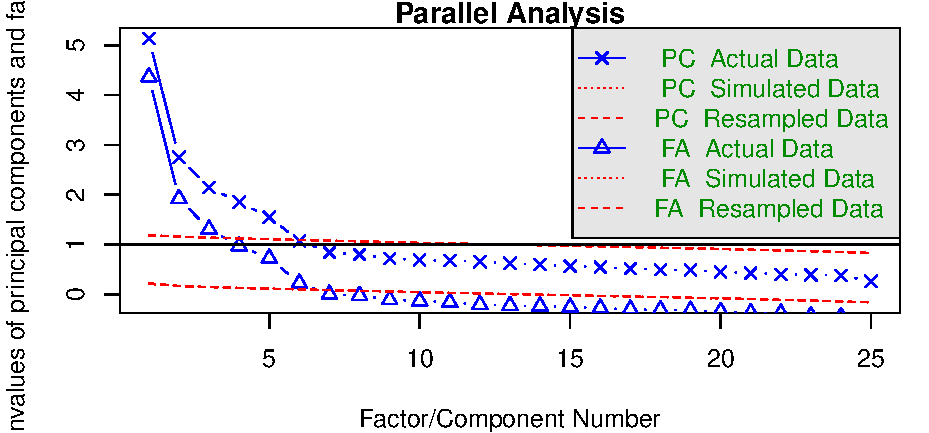
\includegraphics[width=0.45\linewidth,]{fig/Q1plot1-1} 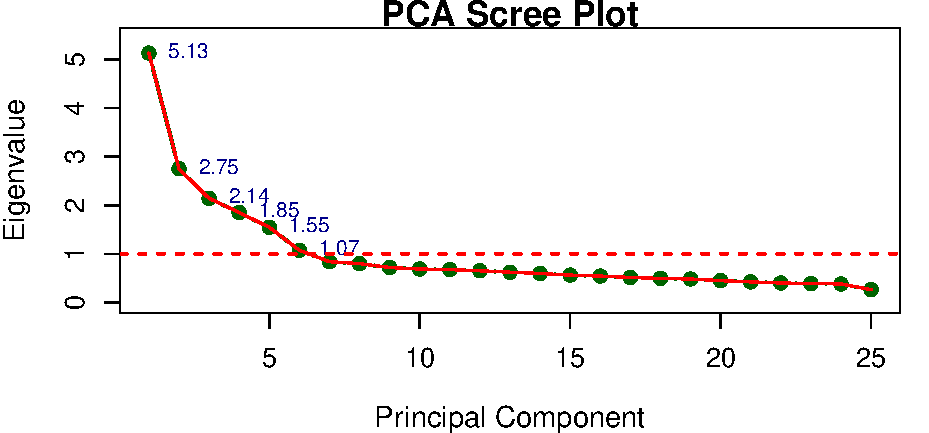
\includegraphics[width=0.45\linewidth,]{fig/Q1plot1-2} 

}

\caption{ parallel analysis and Scree plot for determining the number of factors}\label{fig:Q1plot1}
\end{figure}

Figure \ref{fig:q1plot2} shows the rotated factor loading matrices obtained using varimax and promax rotations. Both rotations produce broadly similar loading patterns, suggesting that the factor structure is stable. Most items load strongly on a single factor, with limited cross-loadings. The promax rotation allows correlations between factors and yields slightly clearer clustering of items. \textbf{Overall, the results support the five-factor solution selected from the scree plot and parallel analysis.}

\begin{figure}[H]

{\centering 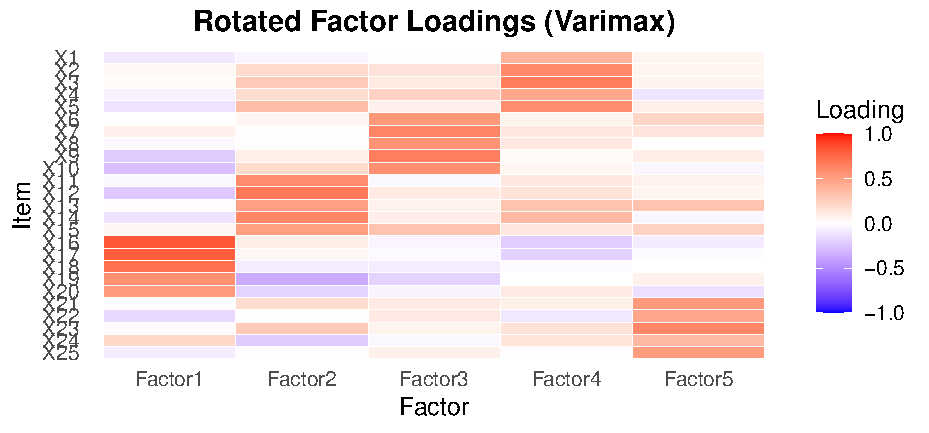
\includegraphics[width=0.45\linewidth,]{fig/q1plot2-1} 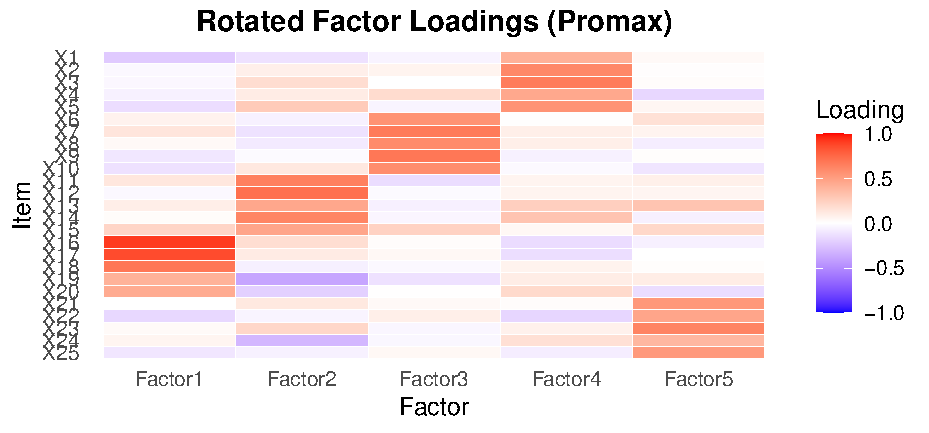
\includegraphics[width=0.45\linewidth,]{fig/q1plot2-2} 

}

\caption{Rotated Factor loadings(Varimax vs Promax)}\label{fig:q1plot2}
\end{figure}

\begin{table}[!h]
\centering
\caption{\label{tab:q1table}Summary of Uniqueness Values}
\centering
\begin{tabular}[t]{cccccc}
\toprule
Min. & 1st Qu. & Median & Mean & 3rd Qu. & Max.\\
\midrule
0.271 & 0.507 & 0.569 & 0.577 & 0.675 & 0.83\\
\bottomrule
\end{tabular}
\end{table}

Table \ref{tab:q1table} showes from 0.27 to 0.83, with an average of approximately 0.58, indicating that the extracted factors explain a moderate proportion of variance in the observed items. The rotated factor loadings reveal a clear five-factor structure. \textbf{Factor 1 loads strongly on items related to emotional instability}(X16--X20), suggesting neuroticism\}. \textbf{Factor 2 reflects extraversion}, with items describing sociability and interpersonal engagement (X11--X15)\}.\textbf{Factor 3 corresponds to conscientiousnes}, capturing organisation, diligence, and careful work behaviour (X6--X10), while \textbf{Factor 4 represents agreeableness}, including empathy and concern for others (X2--X5). Finally, \textbf{Factor 5 is associated with openness to experience}, reflecting intellectual curiosity and reflective thinking (X21--X25).

\newpage

\section{Copula analysis}\label{copula-analysis}

As the majority of claim amounts are zero in the dataset (approximately 93.2\% of 67,856 records), two approaches were initially considered. The first approach retains all observations and models claim amounts using a Tweedie distribution, which accommodates mixed distributions with probability mass at zero. However, this approach could not be implemented because the current GJRM library does not support joint regression combining Poisson frequency with Tweedie severity margins (see Appendix for details). The second approach truncates zero-claim observations and models strictly positive claim amounts using alternative continuous distributions. This is also consistent with actuarial practice, where the focus is typically on modelling positive claims for pricing and reserving purposes. The remainder of Question 2 therefore adopts the second approach.

\subsection{Marginal Distributions Selection}\label{marginal-distributions-selection}

Several truncated count models were considered to account for the absence of zero claims in the dataset, as shown in table \ref{tab:Q2freqPerfTable}. Although the truncated Poisson--Inverse Gaussian specification produces the smallest AIC, the improvement relative to the truncated Poisson model is negligible. (\(\Delta\)AIC \(\approx\) 1.13). The truncated Poisson model is therefore preferred as it achieves the lowest BIC, implying the simplest model.

The fitted model implies represent claim arrivals under the assumption that claims occur independently at a constant rate over the exposure period with an estimated annual claim rate of \(\hat{\mu}=e^{-2.66711}=0.0694\) claims per unit exposure, indicating that claims are relatively infrequent events in the portfolio.

Claim severity was modelled using positive claim amounts only. The distribution of claim costs is strongly right-skewed, which is typical for insurance losses where a small number of claims account for disproportionately large costs. Among the models tested, the Inverse Gaussian distribution provides the best fit, achieving the lowest AIC and BIC values, as shown in table \ref{tab:Q2sevPerfTable}.

The fitted Inverse Gaussian model implies an average positive claim severity of approximately \(\hat{μ}=e^{7.60808} = 2011\), with variability increasing with the cube of the mean, which indicates the heavy right tail commonly observed in claim severity data.

Both graphical and statistical methods are used for model diagnostic. Additional goodness-of-fit tests analysis are in \hyperref[goodness-of-fit-tests]{Goodness-of-fit tests} section of the appendix.
The Q--Q plots obtained from \texttt{res.check()} show that the truncated Poisson model provides a satisfactory representation of claim frequency, while the inverse Gaussian distribution captures the overall shape of the severity distribution. Although the lower tail appears to deviate from the diagonal line, indicating that the model underestimates very small claim amounts, the overall fit is considered adequate for modelling dependence in the following copula analysis. {[}Refer to residual quantile QQ plot of marginal distributions fits here{]}

Convergence diagnostics also indicate stable estimation. In both marginal models the maximum absolute gradient is close to zero, 2.592529e-06 and 9.256606e-13, respectively, and the observed information matrix is positive definite, confirming that the likelihood optimisation has successfully converged.

\subsection{Copula Selection}\label{copula-selection}

To model the dependence between claim frequency and claim severity, four copula families were considered: Gaussian, Student-t, Clayton and Gumbel.
The results are presented in table \ref{tab:copulaPerfTable}.

Among these candidates, the Clayton copula provides the best fit, achieving the lowest AIC and BIC values by a clear margin. Convergence diagnostics confirm stable estimation, with a maximum gradient of \(8.45 \times 10^{-6}\) and a positive definite information matrix.
The estimated Clayton copula parameter is positive and statistically significant \(\theta = 1.47\) , indicating positive dependence between claim frequency and claim severity. It corresponds to a Kendall's \(\tau = \frac{\theta}{(\theta+2)} = 0.4236\), which indicates a moderate positive association between claim frequency and claim severity.
We therefore fit Clayton copula with claytonCopula(param = 1.47, dim = 2).

\subsection{Dependence Interpretation \& Insurance Implication}\label{dependence-interpretation-insurance-implication}

The Clayton copula captures lower-tail dependence, meaning that policies with relatively few claims tend to generate relatively small claim costs. This is reflected in the simulated scatter plot, where observations cluster in the lower-left region of the unit square. Such asymmetric dependence is captured more effectively by the Clayton copula than by symmetric copulas such as the Gaussian or Student-t, which impose identical dependence in both tails.
In contrast, the poorer performance of the Gumbel copula in the previous section suggests weaker upper-tail dependence, meaning that extremely high claim counts are not systematically associated with extremely large claim amounts. This may reflect the heterogeneity of severe claims, where large losses can arise from factors such as accident type or medical costs rather than the number of claims alone.
Overall, the Clayton copula provides a flexible and interpretable representation of the dependence structure between claim frequency and claim severity, capturing the observed lower-tail association while avoiding unrealistic assumptions of symmetric dependence.

\newpage

\subsection{Figures and tables for Q2}\label{figures-and-tables-for-q2}

\begin{table}[!h]
\centering
\caption{\label{tab:Q2freqPerfTable}Claim frequency model performance}
\centering
\begin{tabular}[t]{cccc}
\toprule
Models & df & AIC & BIC\\
\midrule
Truncated Poisson & 1 & 2297.331 & 2303.771\\
Truncated NB I & 1 & 2296.227 & 2309.105\\
Truncated Poisson Inverse Gaussian & 2 & 2296.119 & 2309.077\\
\bottomrule
\end{tabular}
\end{table}

\begin{table}[!h]
\centering
\caption{\label{tab:Q2sevPerfTable}Claim severity model performance}
\centering
\begin{tabular}[t]{cccc}
\toprule
Models & df & AIC & BIC\\
\midrule
LogNormal & 2 & 77708.31 & 77721.19\\
Gamma & 2 & 79329.84 & 79342.72\\
Inverse Gaussian & 2 & 77187.65 & 77200.53\\
\bottomrule
\end{tabular}
\end{table}

\begin{table}[!h]
\centering
\caption{\label{tab:copulaPerfTable}Copula model performance}
\centering
\begin{tabular}[t]{cccc}
\toprule
Models & df & AIC & BIC\\
\midrule
Gaussian & 4 & 79384.86 & 79410.61\\
Student-t & 4 & 79590.55 & 79616.30\\
Clayton & 4 & 79321.95 & 79616.30\\
Gumbel & 4 & 79482.90 & 79508.66\\
\bottomrule
\end{tabular}
\end{table}

\newpage

\section{Principal Component Analysis}\label{principal-component-analysis}

We applied Principal Component Analysis (PCA), an unsupervised dimensionality-reduction method, to transform the 11 variables into a smaller set of uncorrelated components that successively explain the maximum possible variance. Variables were standardised using z-scores before PCA because features are in different units, e.g., income vs age vs rating scores. Without scaling, high-variance variables can dominate PC1 purely due to measurement scale rather than the real underlying structure in the data.

The first three principal components explain approximately 55\% of the total variance, which is sufficient to summarise the main behavioural patterns in the data. Parallel analysis was also examined to determine the appropriate number of components. Although the test suggests retaining two components, the third component still contributes meaningful interpretability and increases the cumulative variance explained. Therefore, three components were retained for further interpretation.

\begin{verbatim}
## Parallel analysis suggests that the number of factors =  3  and the number of components =  3
\end{verbatim}

\begin{figure}[H]

{\centering 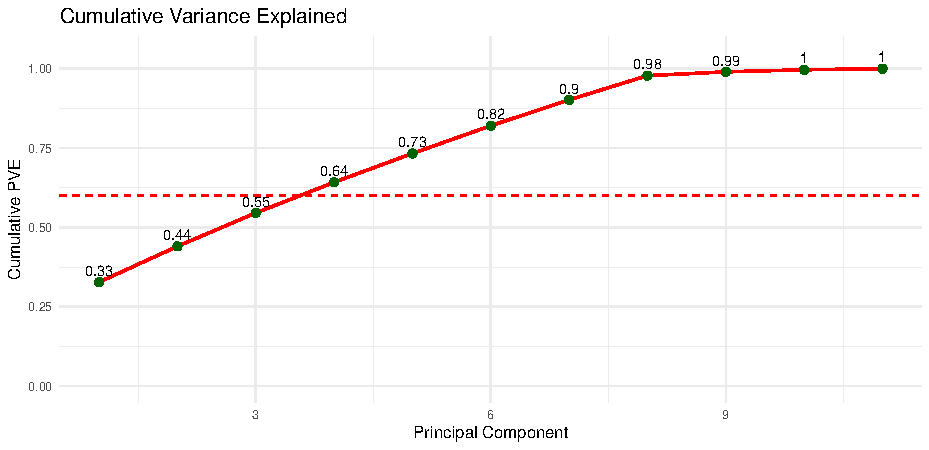
\includegraphics[width=0.45\linewidth,]{fig/Q3plot2-1} 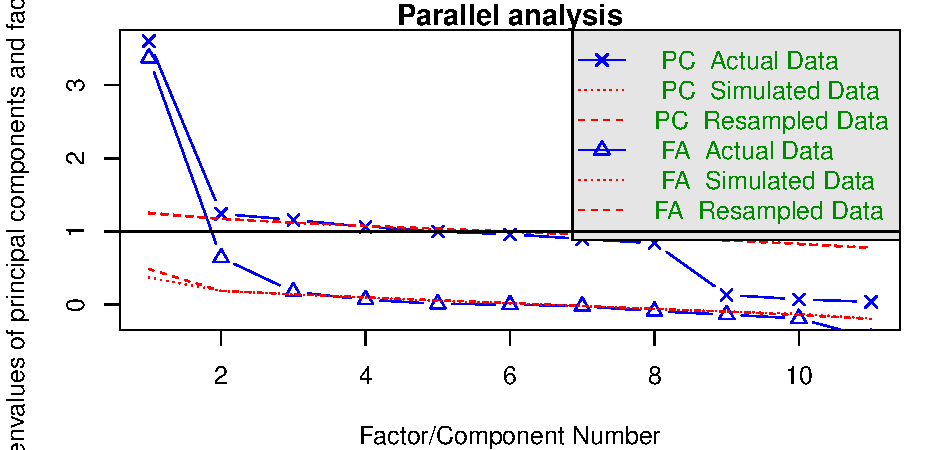
\includegraphics[width=0.45\linewidth,]{fig/Q3plot2-2} 

}

\caption{Cumulative variance, parallel analysis.}\label{fig:Q3plot2}
\end{figure}

The rotated loading plot suggests that RC1 is mainly driven by purchasing behaviour, with income, brand loyalty, shopping frequency, and spending score loading strongly on this component, indicating a dimension of purchasing intensity. RC2 is primarily associated with age and spending score, indicating a contrast between younger high-spending customers and older customers, noting that the sign of loadings is arbitrary. RC3 captures variation in marketing channel engagement: promotion usage and email engagement load positively, whereas social media engagement loads negatively, indicating different preferences across communication channels. Overall, the three rotated components summarise customer behaviour into purchasing intensity, demographic influence, and marketing responsiveness, providing a simplified representation of the main behavioural patterns in the data.

\begin{figure}[H]

{\centering 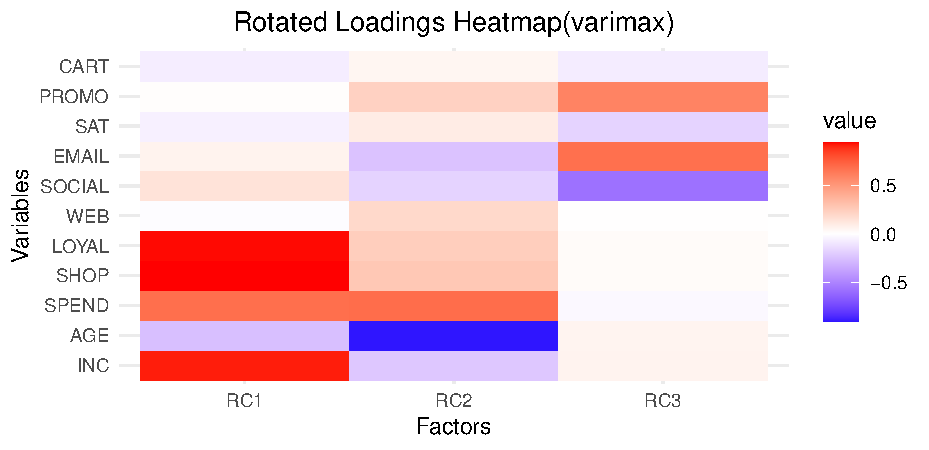
\includegraphics[width=0.45\linewidth,]{fig/Q3plot3-1} 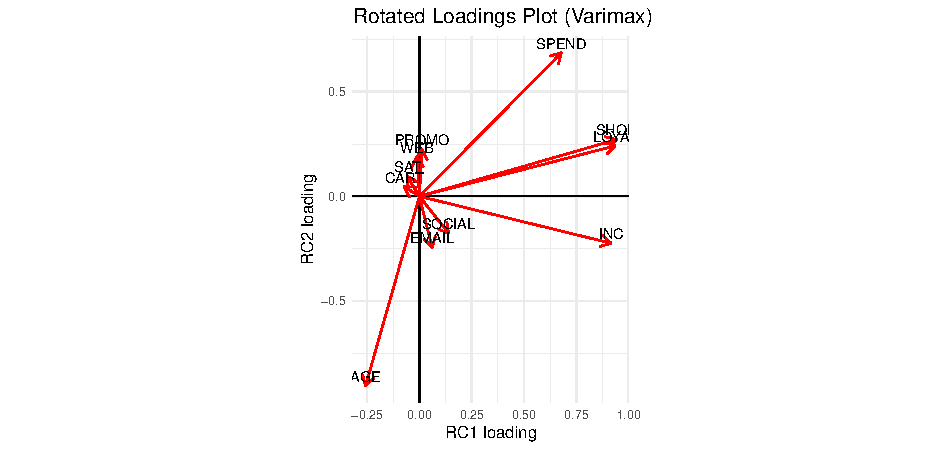
\includegraphics[width=0.45\linewidth,]{fig/Q3plot3-2} 

}

\caption{Heatmap and loading plot of the rotated PCA loadings using varimax rotation.}\label{fig:Q3plot3}
\end{figure}

\begin{table}[!h]
\centering
\caption{\label{tab:q31table}Rotated PCA loadings after varimax rotation (|loading| ≥ 0.40))}
\centering
\resizebox{\ifdim\width>\linewidth\linewidth\else\width\fi}{!}{
\fontsize{9}{11}\selectfont
\begin{tabular}[t]{lccccccccccc}
\toprule
Factor & INC & AGE & SPEND & SHOP & LOYAL & WEB & SOCIAL & EMAIL & SAT & PROMO & CART\\
\midrule
RC1 & 0.92 &  & 0.68 & 0.94 & 0.94 &  &  &  &  &  & \\
RC2 &  & -0.91 & 0.69 &  &  &  &  &  &  &  & \\
RC3 &  &  &  &  &  &  & -0.58 & 0.67 &  & 0.59 & \\
\bottomrule
\end{tabular}}
\end{table}

\newpage

\section{Time series}\label{time-series}

\subsection{Description of time series:}\label{description-of-time-series}

We first plotted the three time series (ts1, ts2 and ts3) and visually assessed the stationarity of each. The plots for ts1 (\ref{fig:q41}) and ts2 suggest they are stationary as they exhibit constant mean and variances, without trend nor seasonality. However, the plot for ts3 suggests non-stationarity with evidence of trend. Formal stationarity test such as Augmented Dickey--Fuller (ADF) tests confirmed these: the p-values for ts3 is large (0.7322), so the null hypothesis of non-stationarity cannot be rejected, whereas the p-values for ts1 and ts2 are smaller than 0.01.

\subsection{Model selection}\label{model-selection}

Model selection heuristics:

\begin{enumerate}
\def\labelenumi{\arabic{enumi}.}
\tightlist
\item
  Use auto.arima to pick p, d, q parameters as a baseline
\item
  Manually fit Arima models for possible combinations of p and q (from 0 to 5 inclusive each), and consider the top 5 models ranked by AIC and BIC.
\item
  Check residuals for models with smaller BIC or AIC than the baseline. The most parsimonious model with satisfactory residuals is then selected.
\end{enumerate}

The final models selected for each time series is:

TS1: (2,0,1) is selected over (2,0,2) suggested by auto.arima because of better AIC and BIC, i.e better fit and simpler.

TS2: (2, 0, 3) as suggested by auto.arima is selected because other models with smaller BIC such as (0, 0, 2), (1, 0, 2) and (1, 0, 2) all exhibit serial correlation according to Ljung-Box tests.

TS3: (2, 1, 0) from auto.arima already has the best AIC and BIC.

\subsection{Model Diagnostics}\label{model-diagnostics}

T1: The diagnostic plots for the fitted ARIMA(2,0,1) model for ts1 are shown in Figure \ref{fig:q43}. The residual ACF and PACF display no significant spikes outside the confidence bounds, suggesting that no substantial autocorrelation remains in the residuals. The Q--Q plot in Figure \ref{fig:q44} indicates that the residuals are approximately normally distributed. In addition, the standardized residuals fluctuate randomly around zero with roughly constant variance. Overall, these diagnostics suggest that the ARIMA(2,0,2) model provides an adequate fit for ts1, as illustrated in Figure \ref{fig:q45}.

T2: The residual diagnostics indicate that most autocorrelations lie within the confidence bounds and the standardized residuals fluctuate randomly around zero. Furthermore, the Q--Q plot in Figure \ref{fig:q47} suggests that the residuals are approximately normally distributed, and overall the diagnostics indicate that the fitted model provides an adequate description of ts2, as shown in Figure \ref{fig:q48}.

T3: The Q--Q plot in Figure \ref{fig:q491} suggests that the residuals are approximately normally distributed. Furthermore, as shown in Figure \ref{fig:q492}, the standardized residuals fluctuate randomly around zero and the residual ACF shows no significant autocorrelation. The Ljung--Box test results also support the conclusion that the residuals behave like white noise, indicating that the fitted model provides an adequate description of the series.

\newpage

\subsection{Figures and tables for Q4}\label{figures-and-tables-for-q4}

\begin{table}[!h]
\centering
\caption{\label{tab:ts1-aicbic}Top 5 ARIMA models for time series 1 ranked by AIC}
\centering
\begin{tabular}[t]{cccc}
\toprule
p & q & AIC & BIC\\
\midrule
2 & 3 & 550.860 & 573.948\\
2 & 4 & 552.701 & 579.087\\
3 & 3 & 552.819 & 579.206\\
4 & 2 & 552.890 & 579.277\\
5 & 5 & 553.855 & 593.435\\
\bottomrule
\end{tabular}
\end{table}

\begin{table}[!h]
\centering
\caption{\label{tab:ts1-aicbic}Top 5 ARIMA models for time series 1 ranked by BIC}
\centering
\begin{tabular}[t]{cccc}
\toprule
p & q & AIC & BIC\\
\midrule
2 & 1 & 554.022 & 570.513\\
1 & 2 & 554.119 & 570.611\\
1 & 1 & 559.434 & 572.627\\
2 & 3 & 550.860 & 573.948\\
2 & 2 & 555.449 & 575.239\\
\bottomrule
\end{tabular}
\end{table}

\begin{table}[!h]
\centering
\caption{\label{tab:ts2-aicbic}Top 5 ARIMA models for time series 2 ranked by AIC}
\centering
\begin{tabular}[t]{cccc}
\toprule
p & q & AIC & BIC\\
\midrule
2 & 4 & 637.204 & 663.591\\
4 & 5 & 637.619 & 673.901\\
3 & 5 & 637.663 & 670.646\\
0 & 2 & 638.011 & 651.204\\
3 & 4 & 638.479 & 668.163\\
\bottomrule
\end{tabular}
\end{table}

\begin{table}[!h]
\centering
\caption{\label{tab:ts2-aicbic}Top 5 ARIMA models for time series 2 ranked by BIC}
\centering
\begin{tabular}[t]{cccc}
\toprule
p & q & AIC & BIC\\
\midrule
0 & 2 & 638.011 & 651.204\\
1 & 2 & 639.797 & 656.289\\
0 & 3 & 639.816 & 656.308\\
2 & 2 & 641.316 & 661.106\\
0 & 4 & 641.493 & 661.283\\
\bottomrule
\end{tabular}
\end{table}

\begin{table}[!h]
\centering
\caption{\label{tab:ts3-aicbic}Top 5 ARIMA models for time series 3 ranked by AIC}
\centering
\begin{tabular}[t]{cccc}
\toprule
p & q & AIC & BIC\\
\midrule
2 & 0 & 555.135 & 565.015\\
2 & 5 & 556.704 & 583.051\\
2 & 1 & 556.830 & 570.003\\
3 & 0 & 556.851 & 570.024\\
5 & 2 & 557.587 & 583.934\\
\bottomrule
\end{tabular}
\end{table}

\begin{table}[!h]
\centering
\caption{\label{tab:ts3-aicbic}Top 5 ARIMA models for time series 3 ranked by BIC}
\centering
\begin{tabular}[t]{cccc}
\toprule
p & q & AIC & BIC\\
\midrule
2 & 0 & 555.135 & 565.015\\
2 & 1 & 556.830 & 570.003\\
3 & 0 & 556.851 & 570.024\\
3 & 1 & 557.974 & 574.441\\
0 & 3 & 561.945 & 575.119\\
\bottomrule
\end{tabular}
\end{table}

\begin{figure}[!ht]

{\centering 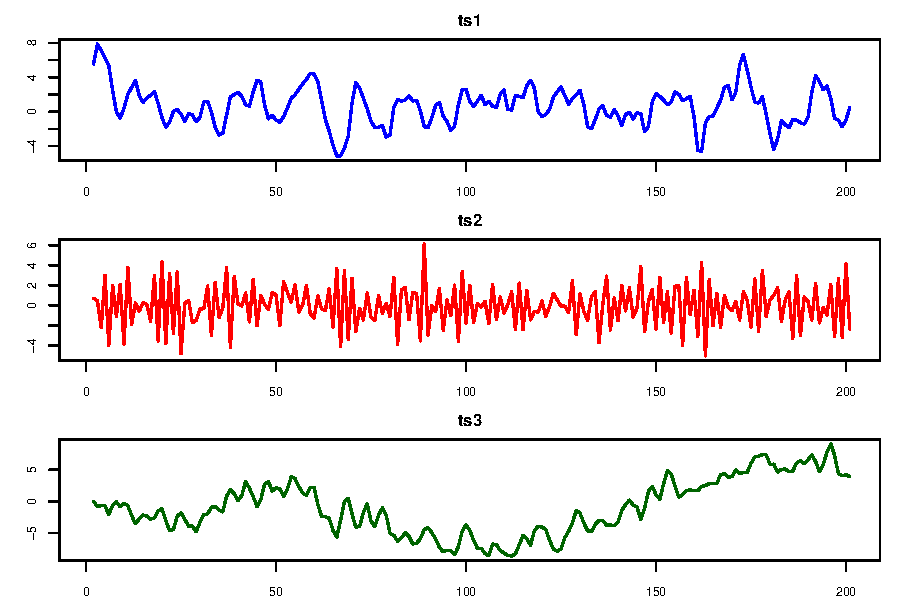
\includegraphics[width=1\linewidth,]{fig/q41-1} 

}

\caption{Time plots of the three simulated series}\label{fig:q41}
\end{figure}

\begin{table}[!h]
\centering
\caption{\label{tab:q42}ADF tests and suggested ARIMA models}
\centering
\begin{tabular}[t]{l|r|r|r}
\hline
Series & ADF\_statistic & p\_value & ARIMA\_model\\
\hline
ts1 & -6.050 & 0.010 & 2\\
\hline
ts2 & -4.108 & 0.010 & 0\\
\hline
ts3 & -1.627 & 0.732 & 2\\
\hline
ts1 & -6.050 & 0.010 & 2\\
\hline
ts2 & -4.108 & 0.010 & 0\\
\hline
ts3 & -1.627 & 0.732 & 3\\
\hline
ts1 & -6.050 & 0.010 & 2\\
\hline
ts2 & -4.108 & 0.010 & 1\\
\hline
ts3 & -1.627 & 0.732 & 0\\
\hline
\end{tabular}
\end{table}

\begin{figure}[H]

{\centering 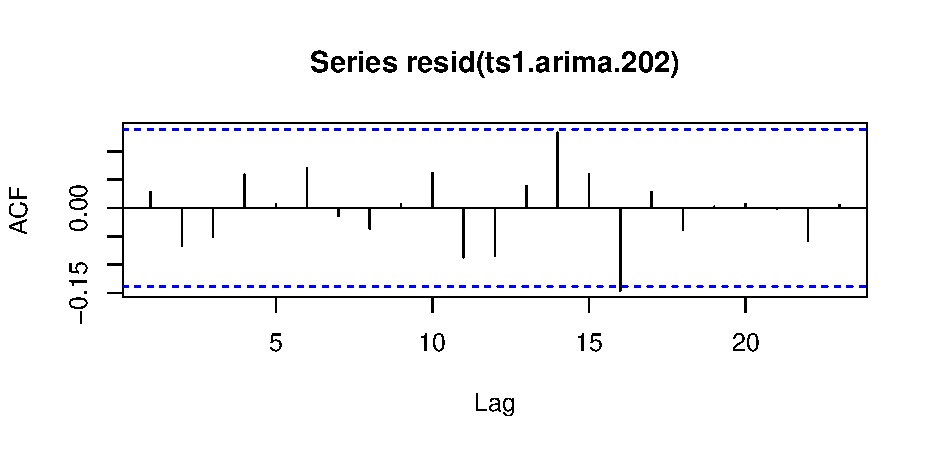
\includegraphics[width=0.45\linewidth,]{fig/q43-1} 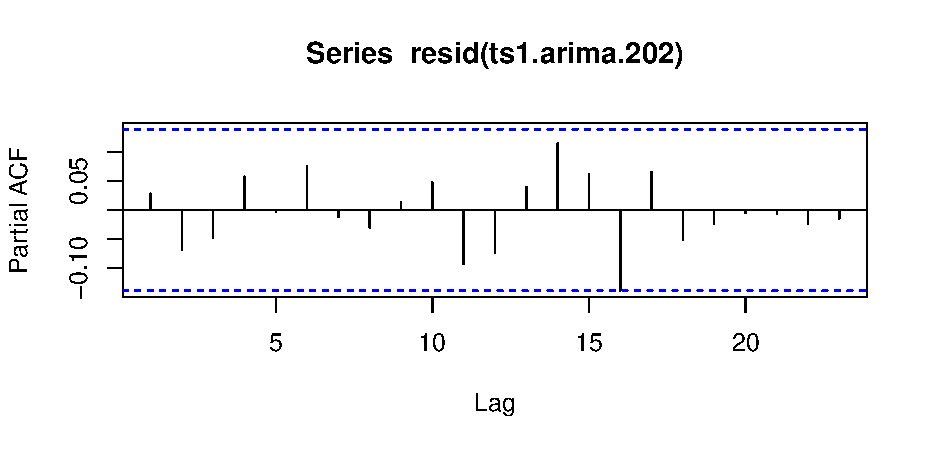
\includegraphics[width=0.45\linewidth,]{fig/q43-2} 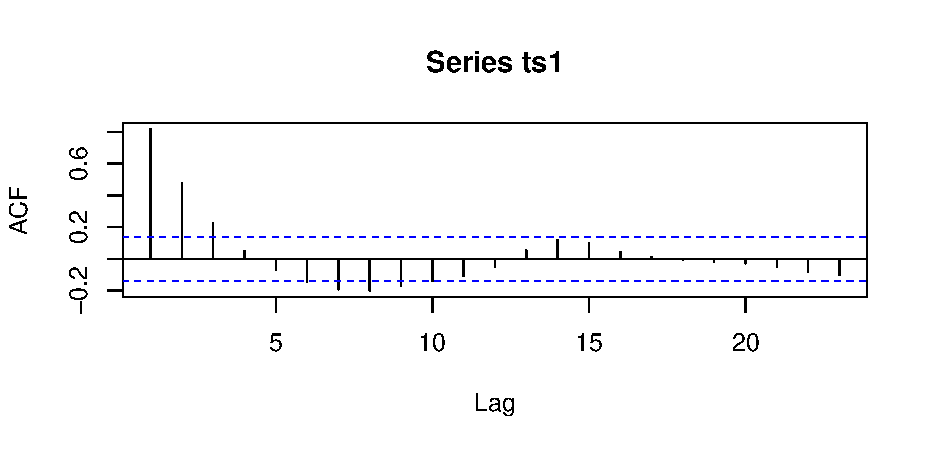
\includegraphics[width=0.45\linewidth,]{fig/q43-3} 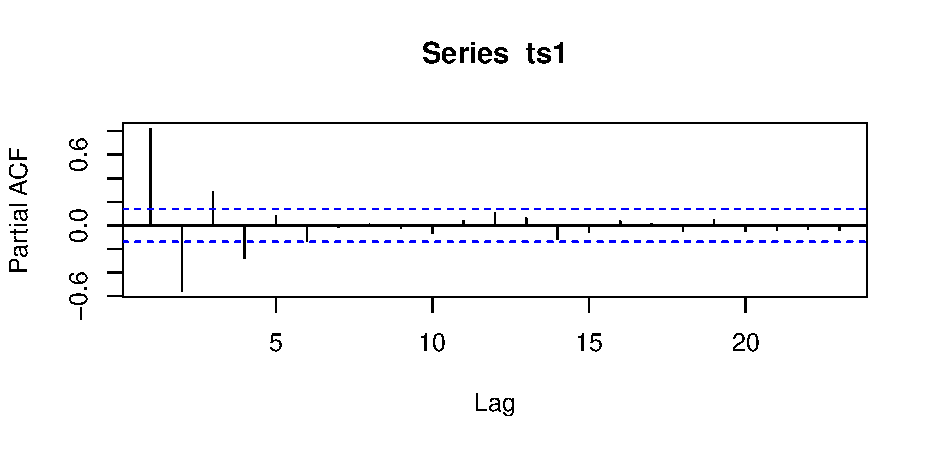
\includegraphics[width=0.45\linewidth,]{fig/q43-4} 

}

\caption{ACF vs PACF}\label{fig:q43}
\end{figure}

\begin{figure}[H]

{\centering 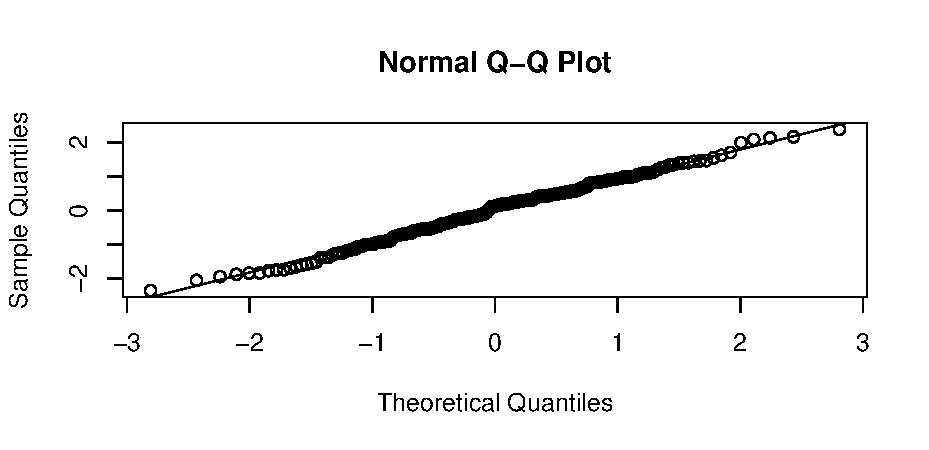
\includegraphics[width=0.9\linewidth,]{fig/q44-1} 

}

\caption{QQPLOT}\label{fig:q44}
\end{figure}

\begin{figure}[H]

{\centering 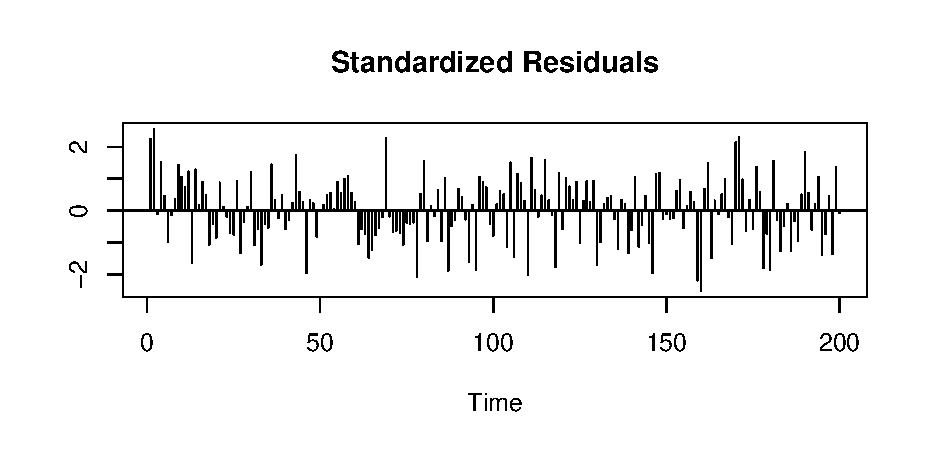
\includegraphics[width=0.45\linewidth,]{fig/q45-1} 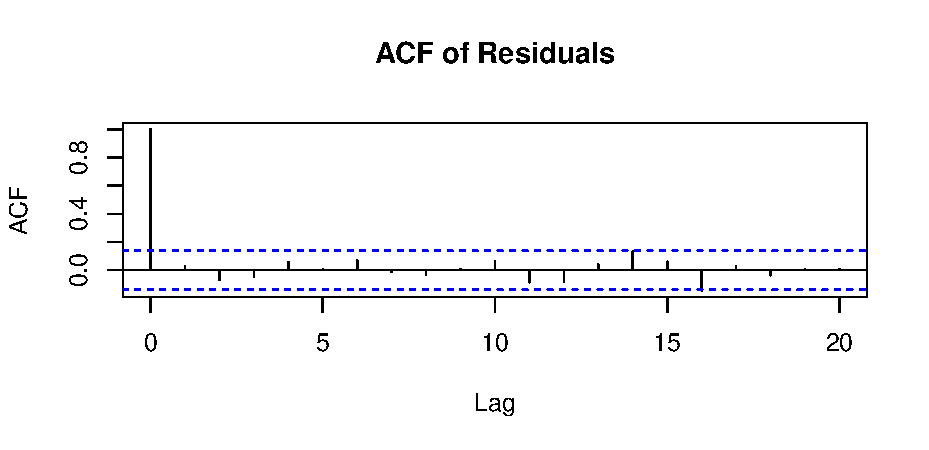
\includegraphics[width=0.45\linewidth,]{fig/q45-2} 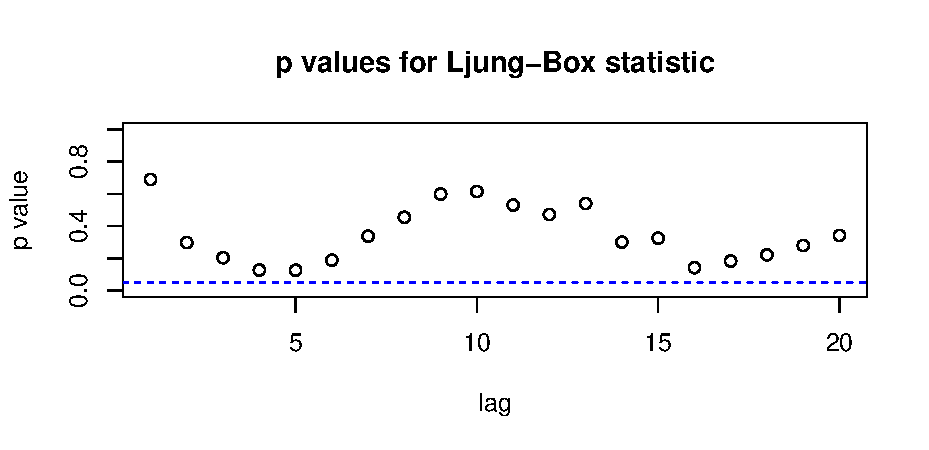
\includegraphics[width=0.45\linewidth,]{fig/q45-3} 

}

\caption{Diagnostic plots for the fitted ARIMA(2,0,2) model for ts1, including standardized residuals, residual ACF, and Ljung–Box test results.}\label{fig:q45}
\end{figure}

\begin{figure}[H]

{\centering 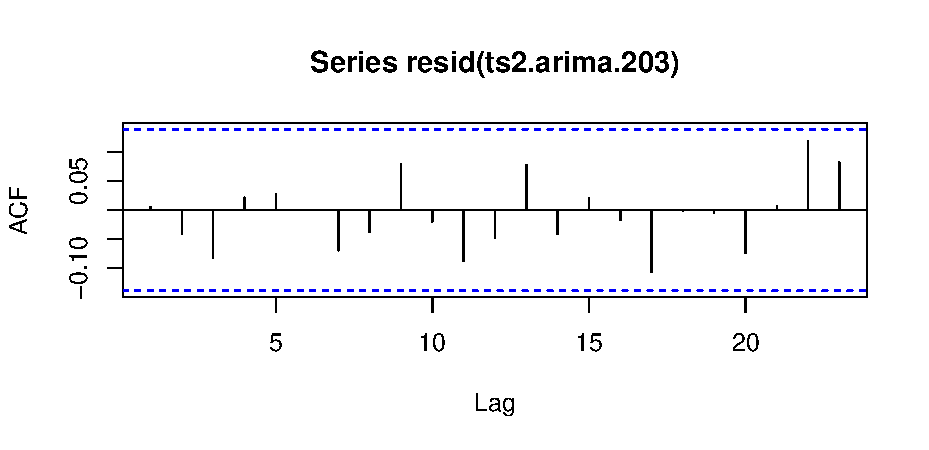
\includegraphics[width=0.45\linewidth,]{fig/q46-1} 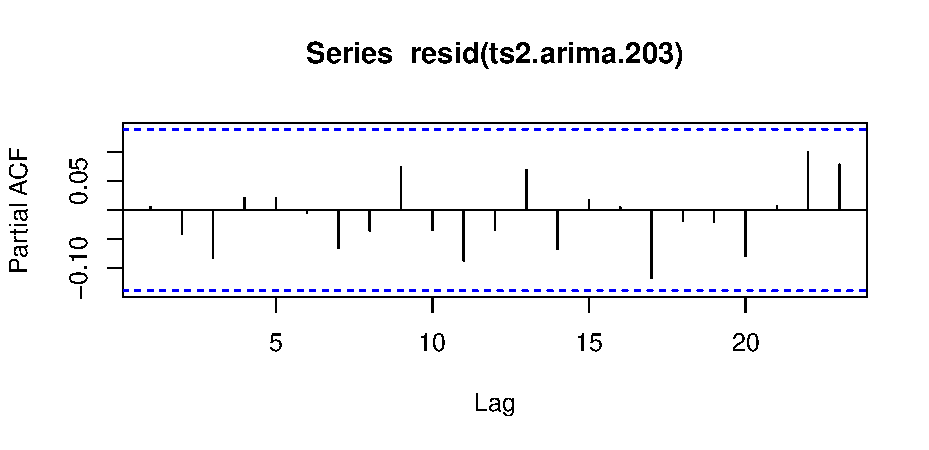
\includegraphics[width=0.45\linewidth,]{fig/q46-2} 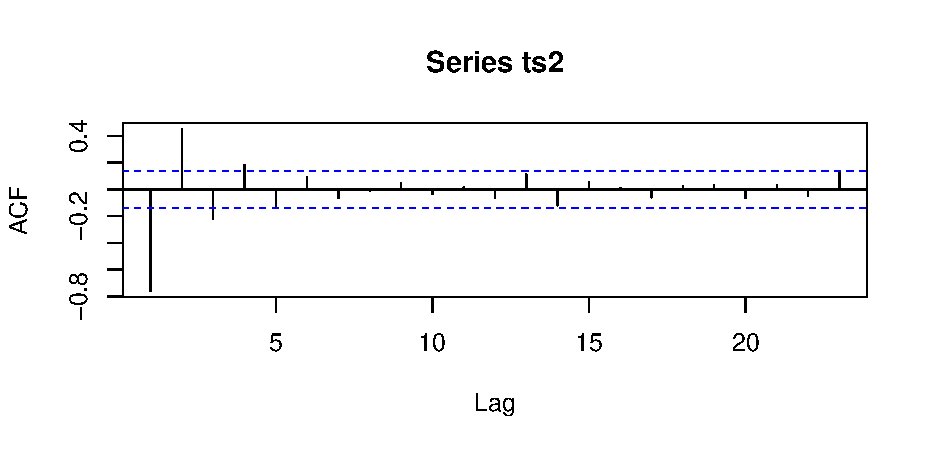
\includegraphics[width=0.45\linewidth,]{fig/q46-3} 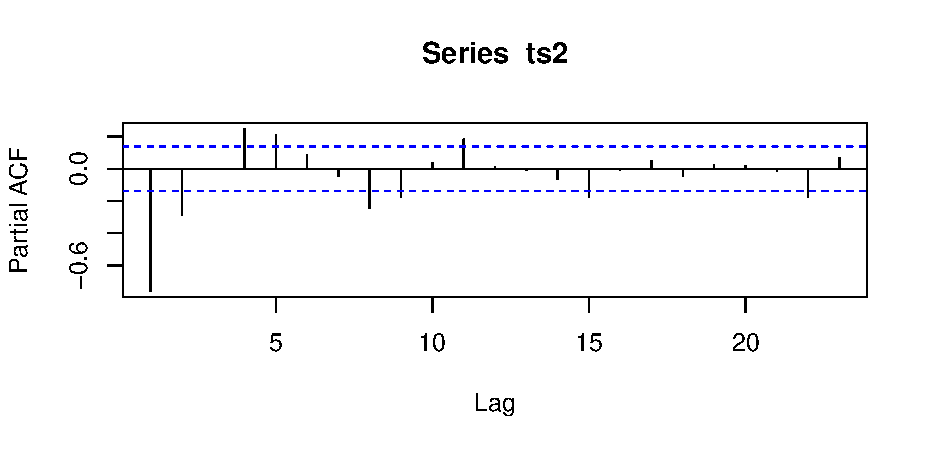
\includegraphics[width=0.45\linewidth,]{fig/q46-4} 

}

\caption{ACF vs PACF}\label{fig:q46}
\end{figure}

\begin{figure}[H]

{\centering 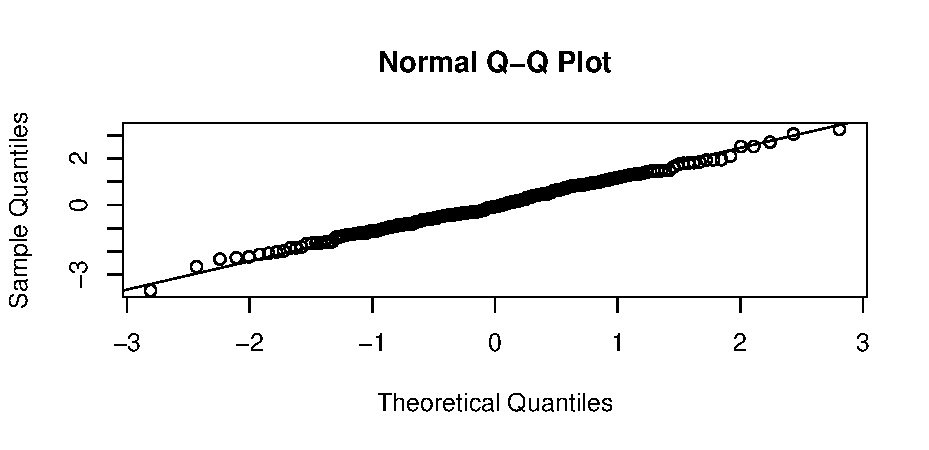
\includegraphics[width=0.9\linewidth,]{fig/q47-1} 

}

\caption{QQPLOT}\label{fig:q47}
\end{figure}

\begin{figure}[H]

{\centering 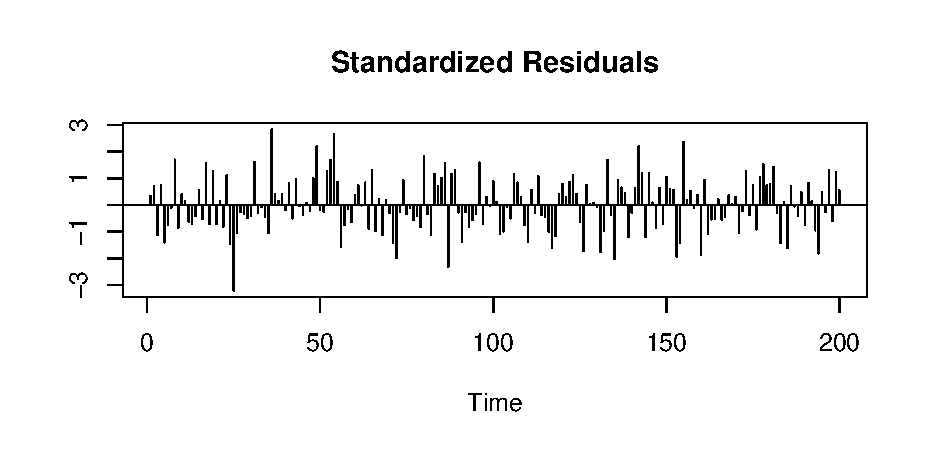
\includegraphics[width=0.45\linewidth,]{fig/q48-1} 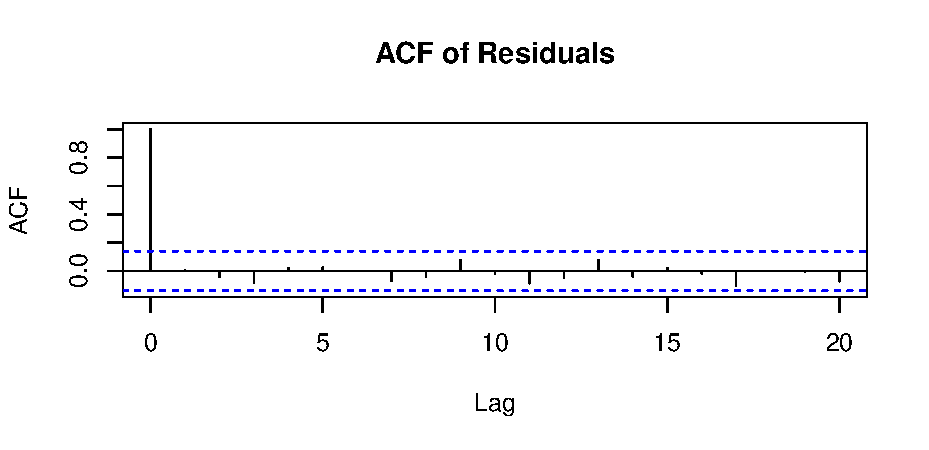
\includegraphics[width=0.45\linewidth,]{fig/q48-2} 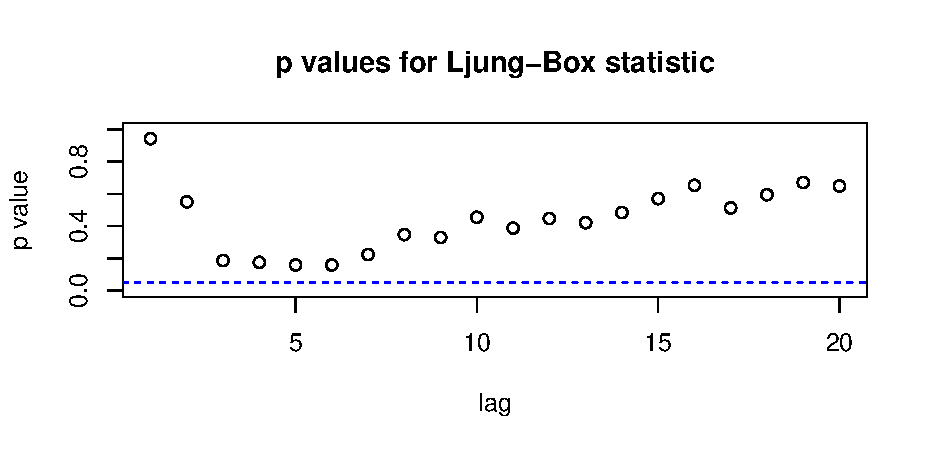
\includegraphics[width=0.45\linewidth,]{fig/q48-3} 

}

\caption{Diagnostic plots for the fitted ARIMA(2,0,3) model for ts2, including standardized residuals, residual ACF, and Ljung–Box test results.}\label{fig:q48}
\end{figure}

\begin{figure}[H]

{\centering 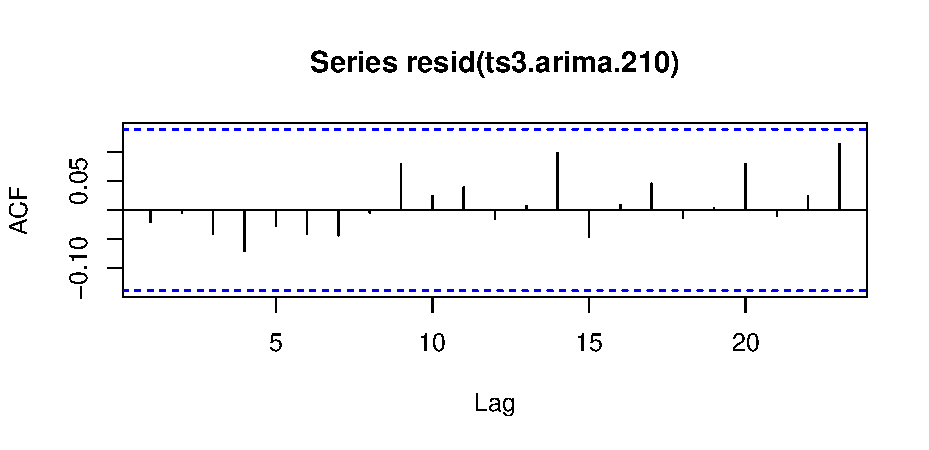
\includegraphics[width=0.45\linewidth,]{fig/q49-1} 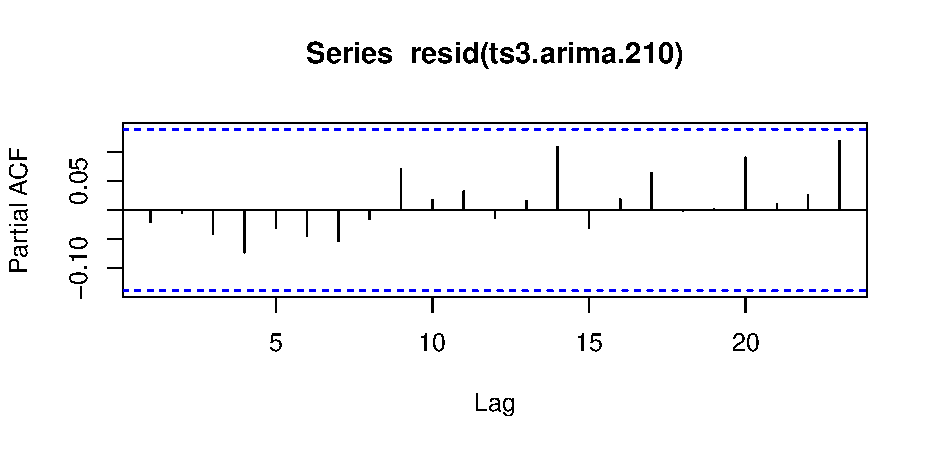
\includegraphics[width=0.45\linewidth,]{fig/q49-2} 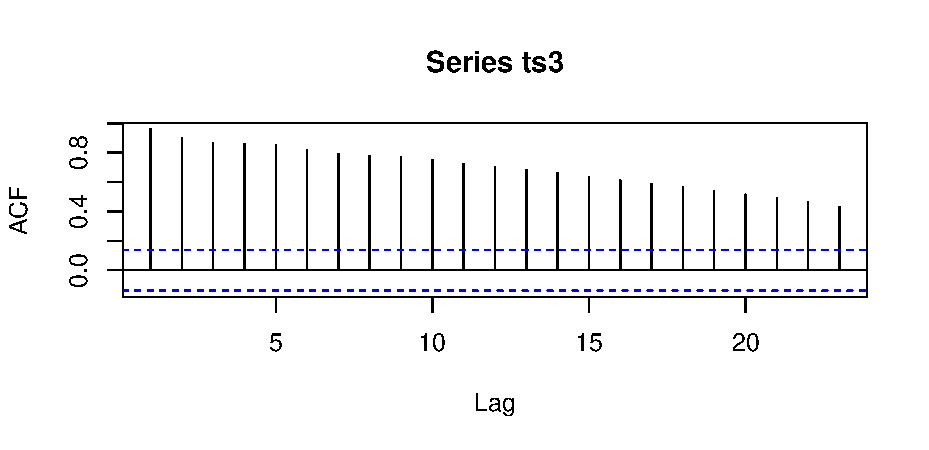
\includegraphics[width=0.45\linewidth,]{fig/q49-3} 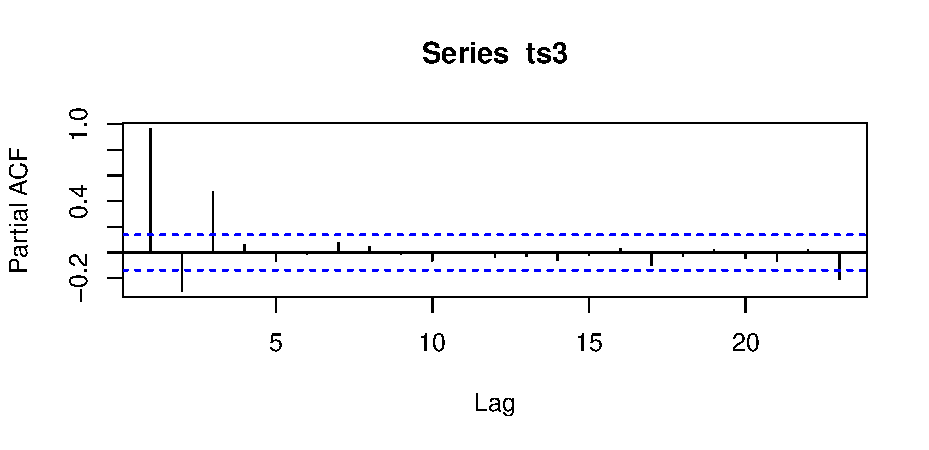
\includegraphics[width=0.45\linewidth,]{fig/q49-4} 

}

\caption{ACF vs PACF}\label{fig:q49}
\end{figure}

\begin{figure}[H]

{\centering 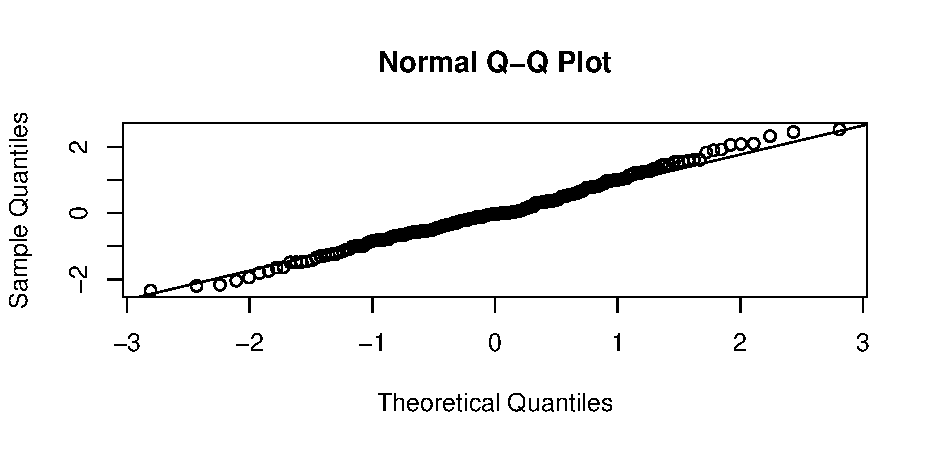
\includegraphics[width=0.9\linewidth,]{fig/q491-1} 

}

\caption{QQPLOT}\label{fig:q491}
\end{figure}

\begin{figure}[H]

{\centering 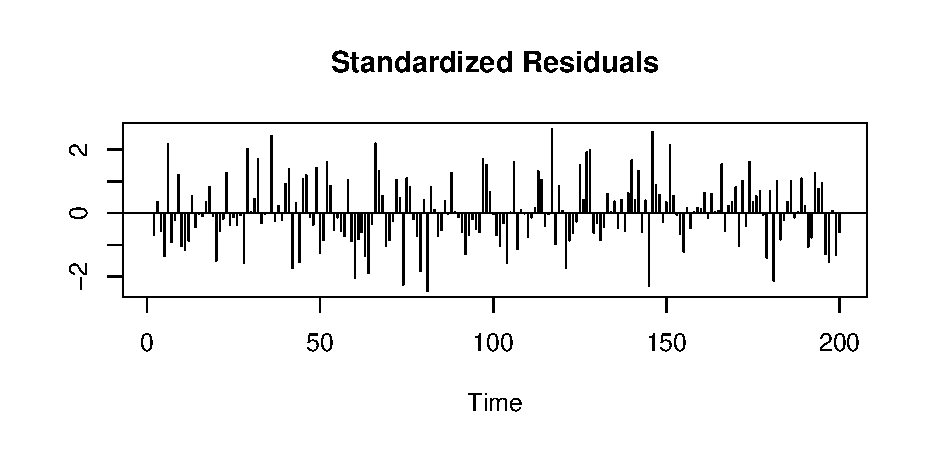
\includegraphics[width=0.45\linewidth,]{fig/q492-1} 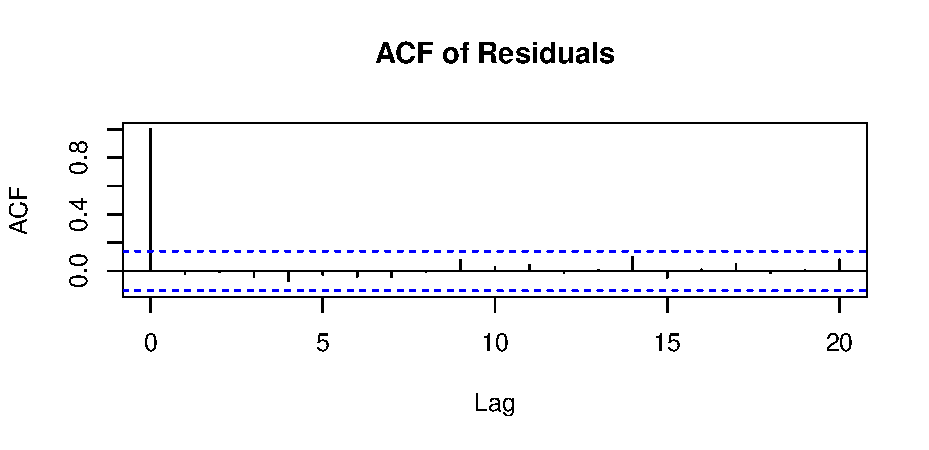
\includegraphics[width=0.45\linewidth,]{fig/q492-2} 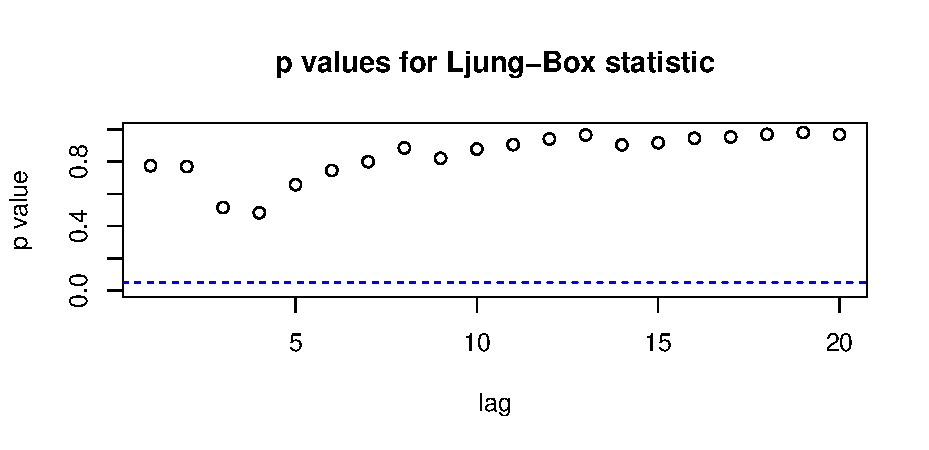
\includegraphics[width=0.45\linewidth,]{fig/q492-3} 

}

\caption{Diagnostic plots for the fitted ARIMA(2,1,0) model for ts3, including standardized residuals, residual ACF, and Ljung–Box test results.}\label{fig:q492}
\end{figure}

\newpage

\section{Appendix}\label{appendix}

\subsection{bonus : Q1 Factor analysis comparison(number of factors 5 vs 6)}\label{bonus-q1-factor-analysis-comparisonnumber-of-factors-5-vs-6}

The heatmaps compare the rotated factor loading structures obtained from the five-factor and six-factor solutions using varimax rotation. In the five-factor solution, items generally load strongly on a single factor, producing a relatively clear and interpretable structure. When a sixth factor is introduced, several items show weaker or more dispersed loadings across factors, suggesting a less stable structure. In particular, the additional sixth factor captures only a limited number of items and does not form a clearly interpretable dimension. Therefore, the five-factor solution appears more parsimonious and provides a more coherent representation of the underlying personality traits.

\begin{figure}[H]

{\centering 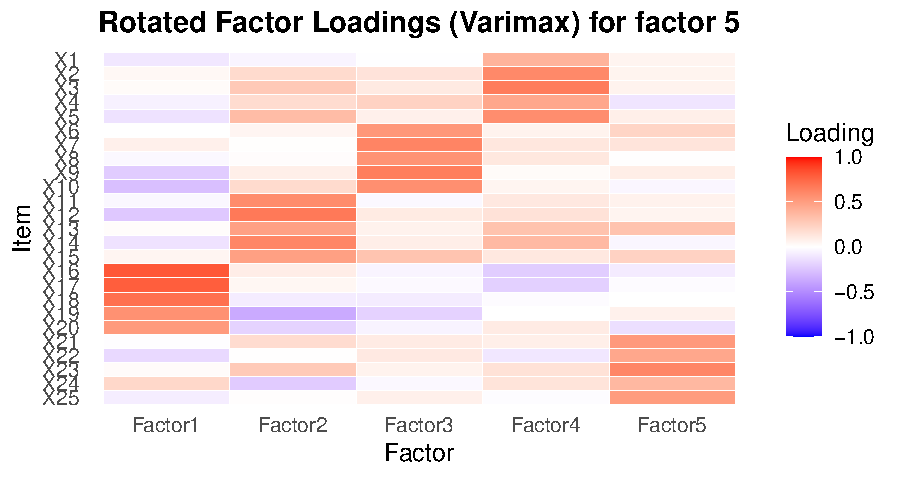
\includegraphics[width=0.45\linewidth,]{fig/appq1-1} 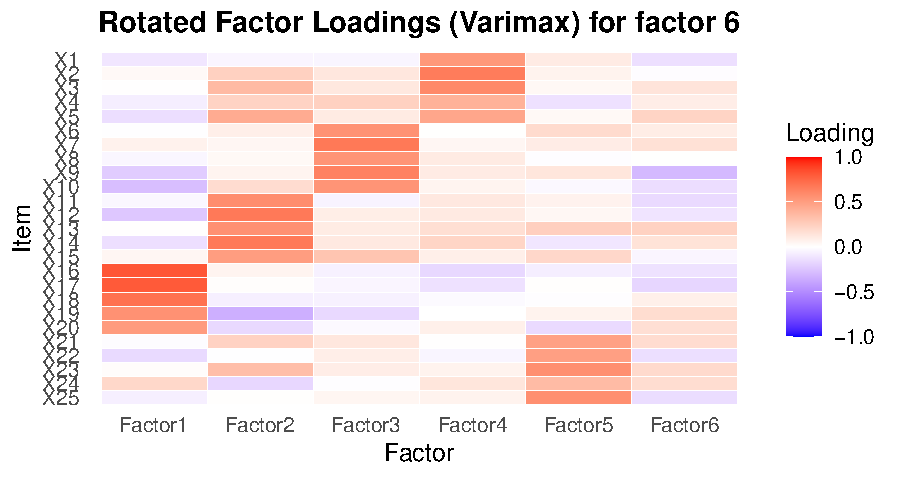
\includegraphics[width=0.45\linewidth,]{fig/appq1-2} 

}

\caption{Comparison of the number of factors (5 vs 6)}\label{fig:appq1}
\end{figure}

The rotated factor loading tables allow a comparison between the five-factor and six-factor solutions. In the five-factor model, the items cluster clearly into five interpretable groups, with most salient loadings above 0.40 concentrated on a single factor. In contrast, the six-factor solution does not substantially improve the structure, as the additional sixth factor (F6) does not show any strong loadings above the threshold. Most items continue to load on the same factors as in the five-factor solution, indicating that the extra factor does not capture a distinct dimension. Therefore, the five-factor model appears more parsimonious and provides a clearer and more interpretable representation of the underlying personality structure.

\begin{table}[!h]
\centering
\caption{\label{tab:appq1table}Rotated Factor Loadings for 5 Factors (|loading| ≥ 0.40)}
\centering
\resizebox{\ifdim\width>\linewidth\linewidth\else\width\fi}{!}{
\fontsize{9}{11}\selectfont
\begin{tabular}[t]{lccccccccccccccccccccccccc}
\toprule
Factor & X1 & X2 & X3 & X4 & X5 & X6 & X7 & X8 & X9 & X10 & X11 & X12 & X13 & X14 & X15 & X16 & X17 & X18 & X19 & X20 & X21 & X22 & X23 & X24 & X25\\
\midrule
F1 &  &  &  &  &  &  &  &  &  &  &  &  &  &  &  & 0.82 & 0.79 & 0.71 & 0.56 & 0.52 &  &  &  &  & \\
F2 &  &  &  &  &  &  &  &  &  &  & 0.59 & 0.67 & 0.49 & 0.61 & 0.49 &  &  &  &  &  &  &  &  &  & \\
F3 &  &  &  &  &  & 0.53 & 0.62 & 0.55 & 0.65 & 0.57 &  &  &  &  &  &  &  &  &  &  &  &  &  &  & \\
F4 &  & 0.60 & 0.66 & 0.45 & 0.58 &  &  &  &  &  &  &  &  &  &  &  &  &  &  &  &  &  &  &  & \\
F5 &  &  &  &  &  &  &  &  &  &  &  &  &  &  &  &  &  &  &  &  & 0.52 & 0.45 & 0.61 &  & 0.51\\
\bottomrule
\end{tabular}}
\end{table}

\begin{table}[!h]
\centering
\caption{\label{tab:appq2table}Rotated Factor Loadings for 6 Factors (|loading| ≥ 0.40)}
\centering
\resizebox{\ifdim\width>\linewidth\linewidth\else\width\fi}{!}{
\fontsize{9}{11}\selectfont
\begin{tabular}[t]{lccccccccccccccccccccccccc}
\toprule
Factor & X1 & X2 & X3 & X4 & X5 & X6 & X7 & X8 & X9 & X10 & X11 & X12 & X13 & X14 & X15 & X16 & X17 & X18 & X19 & X20 & X21 & X22 & X23 & X24 & X25\\
\midrule
F1 &  &  &  &  &  &  &  &  &  &  &  &  &  &  &  & 0.82 & 0.81 & 0.71 & 0.56 & 0.51 &  &  &  &  & \\
F2 &  &  &  &  & 0.44 &  &  &  &  &  & 0.58 & 0.67 & 0.57 & 0.67 & 0.51 &  &  &  &  &  &  &  &  &  & \\
F3 &  &  &  &  &  & 0.56 & 0.68 & 0.55 & 0.64 & 0.55 &  &  &  &  &  &  &  &  &  &  &  &  &  &  & \\
F4 & 0.53 & 0.66 & 0.60 & 0.40 & 0.46 &  &  &  &  &  &  &  &  &  &  &  &  &  &  &  &  &  &  &  & \\
F5 &  &  &  &  &  &  &  &  &  &  &  &  &  &  &  &  &  &  &  &  & 0.48 & 0.49 & 0.57 &  & 0.57\\
\addlinespace
F6 &  &  &  &  &  &  &  &  &  &  &  &  &  &  &  &  &  &  &  &  &  &  &  &  & \\
\bottomrule
\end{tabular}}
\end{table}

\newpage

\subsection{bonus : Q2 Copula}\label{bonus-q2-copula}

\subsubsection{Goodness-of-fit tests}\label{goodness-of-fit-tests}

Goodness-of-fit tests were conducted using the Kolmogorov--Smirnov (KS) and Cramér--von Mises (CvM) statistics. Null hypothesis is data follow the fitted marginal distribution.The KS statistic (D1=0.93707, D2=0.74048) measures the maximum difference between the empirical and theoretical cumulative distributions of zero truncated poisson and inverse gaussian, while the Cramér--von Mises statistic (\(\omega_1^2 =1268.4\), \(\omega_1^2=653.09\)) measures the overall squared discrepancy across two distributions. Both tests reject the null hypothesis that the observed data follow the fitted distributions exactly (p-value \textless{} \(2.2 \times 10^{-16}\)). However, with a sample size of n = 4624, these tests are highly sensitive and may detect even minor deviations from the theoretical distribution.

\subsubsection{Adding covariates into the models}\label{adding-covariates-into-the-models}

Additional models including covariates were explored to assess whether observable policy characteristics improve the marginal model specification. In particular, vehicle value, geographic area and gender were considered, as these variables may plausibly influence accident risk and claim costs. For example, vehicle value may affect repair costs, while area and gender may capture differences in driving behaviour or traffic exposure. In the claim frequency model, the intercept-only truncated Poisson specification achieves the lowest AIC and BIC compared to models with extra covariates. For the claim severity model, the inclusion of 4 extra covariates, including vehicle value, area and gender producing the lowest AIC. However, BIC again favours the simpler intercept-only specification. Overall, it is suggested that the additional covariates provide limited explanatory power in this dataset.

{[}Put table here{]}
{[}Put link in the main articles{]}

\newpage

\subsection{bonus : Q3 Principal Component Analysis}\label{bonus-q3-principal-component-analysis}

The correlation matrix shows generally weak to moderate correlations among variables, suggesting that several variables related to purchasing behaviour (spending score, Shopping Frequency, and Brand loyalty) are strongly positively correlated. PC1 contrasts purchasing intensity (spending score, shopping frequency, and brand loyalty) against age, suggesting that older customers tend to have lower purchasing-intensity scores on this component( here can add scatterplot as evidence to support if have space).

\begin{figure}[H]

{\centering 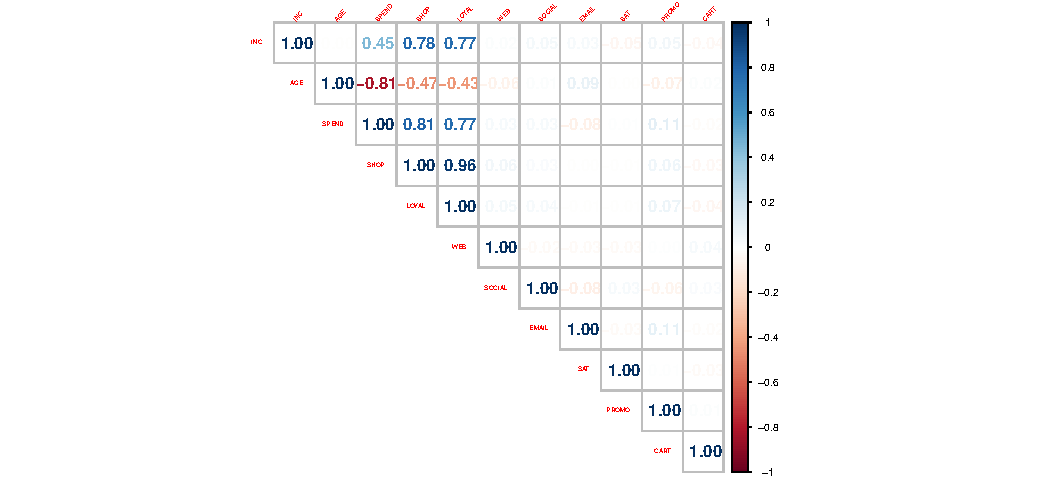
\includegraphics[width=0.45\linewidth,]{fig/Q3Cor-1} 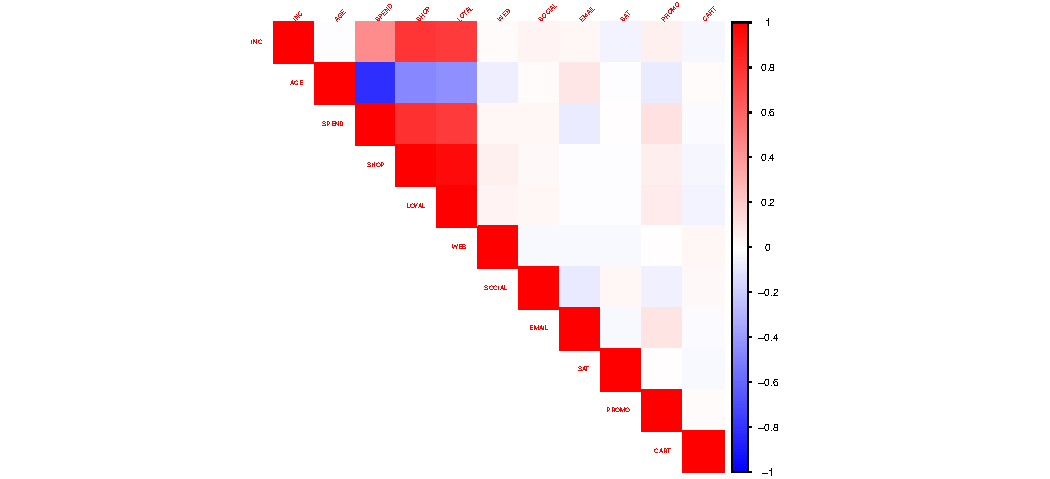
\includegraphics[width=0.45\linewidth,]{fig/Q3Cor-2} 

}

\caption{Correlation matrix (numbers left, heatmap right)}\label{fig:Q3Cor}
\end{figure}

The scree plot suggests retaining three to four components. Although the Kaiser criterion indicates four components (eigenvalue \textgreater{} 1), the elbow in the scree plot and the interpretability of the rotated loadings support retaining three components.

\begin{figure}[H]

{\centering 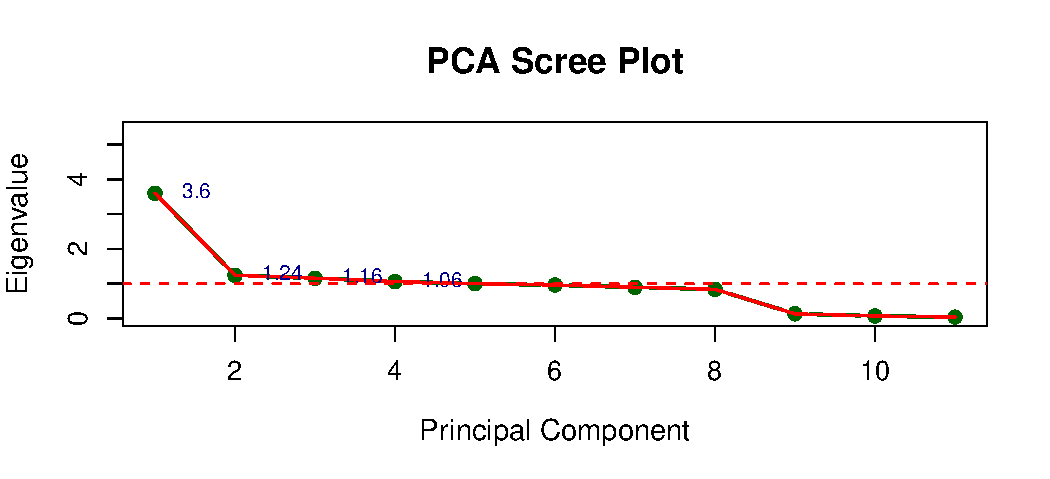
\includegraphics[width=1\linewidth,]{fig/Q3screeplot-1} 

}

\caption{Scree plot}\label{fig:Q3screeplot}
\end{figure}

The scatter plot shows the distribution of observations in the space of the first two principal components, with clusters identified using k-means clustering. The results suggest three groups of customers with different behavioural patterns. One group is associated with higher purchasing intensity (high PC1 values), while another group corresponds to lower purchasing activity. The third group lies between these extremes, representing customers with moderate purchasing behaviour.

\begin{figure}[H]

{\centering 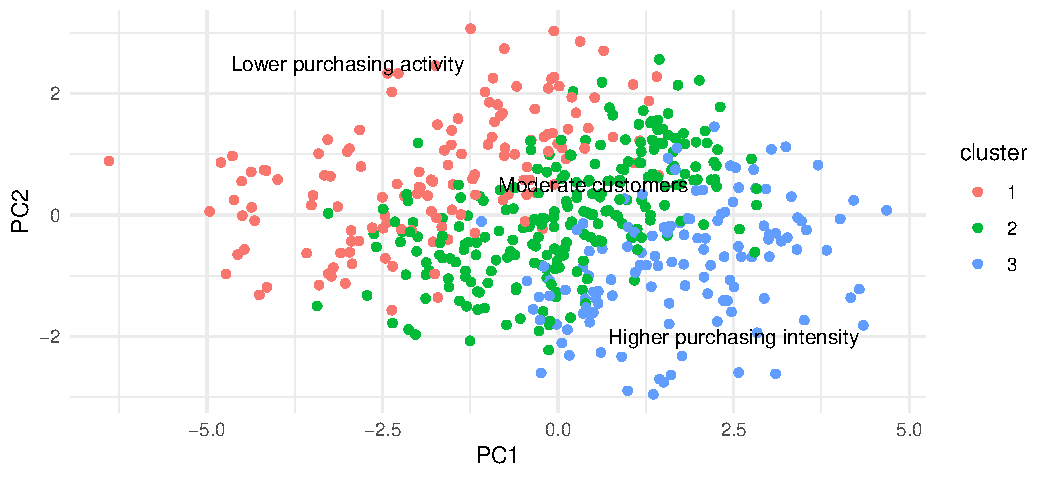
\includegraphics[width=1\linewidth,]{fig/Q3clusterlot-1} 

}

\caption{Scatter plot}\label{fig:Q3clusterlot}
\end{figure}

The PCA biplot illustrates both the observations and the directions of the original variables in the space of the first two principal components. Variables related to purchasing behaviour, such as income, brand loyalty, shopping frequency, and spending score, are largely aligned with the direction of PC1, indicating their strong contribution to this component. In contrast, age is oriented in a different direction, suggesting that it captures a different aspect of variation in the data. Overall, the biplot confirms that purchasing-related variables primarily drive the variation explained by the first principal component.

\begin{figure}[H]

{\centering 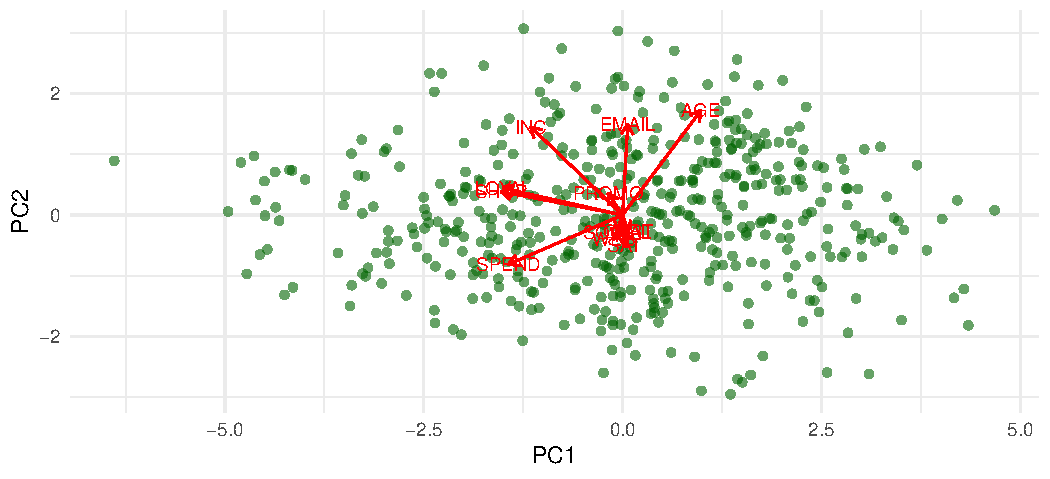
\includegraphics[width=1\linewidth,]{fig/Q3biplot-1} 

}

\caption{PCA Biplot}\label{fig:Q3biplot}
\end{figure}

The three-dimensional PCA score plot provides a visual representation of the observations across the first three principal components. The points form a continuous distribution rather than clearly separated clusters, indicating that customer behaviour varies gradually across the dataset. This visualization further supports the interpretation that the main variation in the data is captured by the first few principal components.

\begin{figure}[!ht]

{\centering 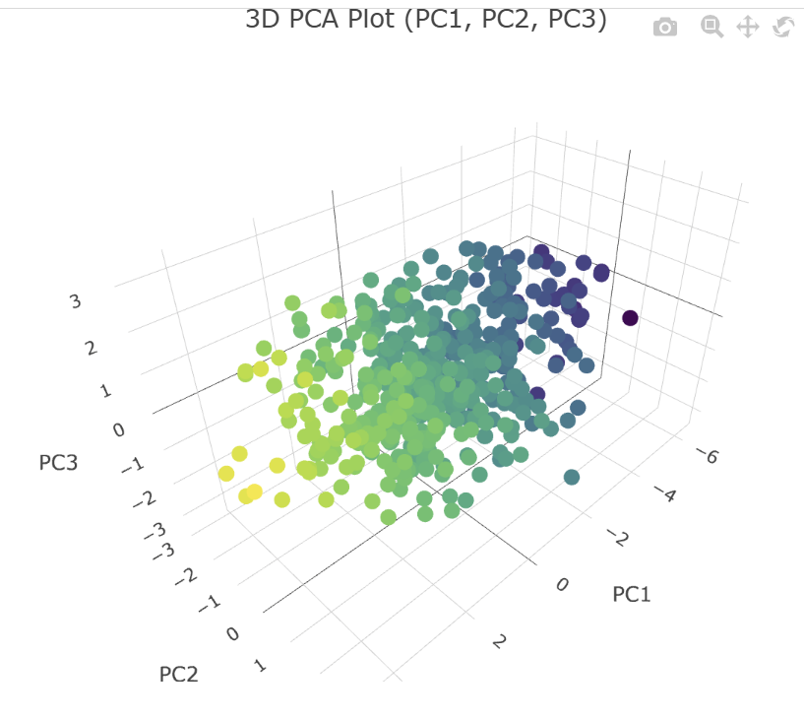
\includegraphics[width=0.8\linewidth,]{fig/principal3d} 

}

\caption{3D PCA score plot of the first three principal components. }\label{fig:principal3d}
\end{figure}

\newpage

\subsection{bonus : Q4 Time series}\label{bonus-q4-time-series}

\end{document}
